\documentclass[cheatsheet.tex]{subfiles}
\begin{document}
multi-class contingency table,  confusion matrix. 
\textbullet One-versus-rest scheme, learn k-1 models, apply in sequence \textbullet One-versus-rest scheme, learn a one-class model for each class \textbullet One-versus-one scheme, learn a model for each pair of classes \textbullet One-versus-one scheme with a decision tree
\subsection{Multi-Classification}
\textbf{K-class classifiers:} Combine several binary classifiers to build it:\textbullet learn k-1 models, apply in sequence \textbullet learn a one-class model for each class \textbullet learn a model for each pair of classes, Train k (k-1)/2 binary classifiers, apply them all to \textbf{x} and vote \textbullet with a decision tree
\\
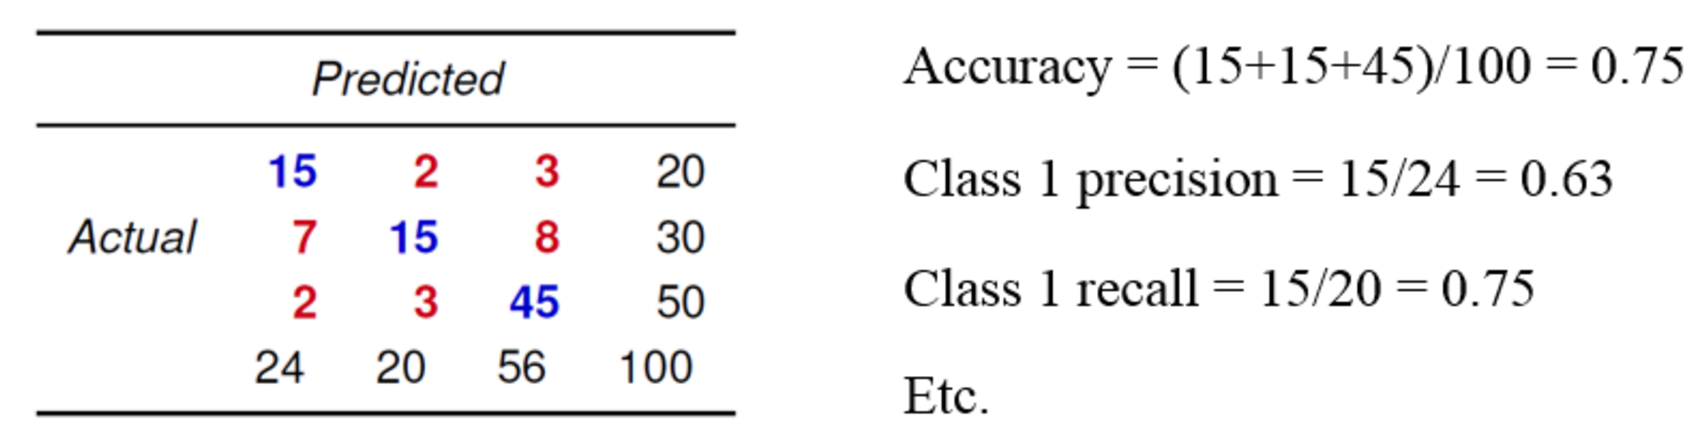
\includegraphics[width=80mm]{confusion_matrix.png}
\subsection{Regression}
\textbf{Regression is another predictive ML task}, learns a function: $\hat{f} : x \rightarrow R$ from examples - $f(x_i)$ \textbullet If fitting N-degree polynomial, choose one as low degree as possible to prevent overfitting. \textbullet The number of data points should be much greater than the number of parameters to be estimated. \textbullet \textbf{Residual:} $r(x)=f(x)-\hat{f}(x)$ \textbullet \textbf{loss function L} $L(x)=r^2(x)=(f(x)-\hat{f}(x))^2$
\subsection{Unsupervised \& Descriptive learning}
skipped
\end{document}